\documentclass[12pt]{article}
\usepackage{blindtext}
\usepackage[en,bordered]{uni-style}
\usepackage{uni-math}
\usepackage{physics}
\usepackage{amssymb}
\usepackage{capt-of}
\DeclareMathOperator*{\argmax}{arg\,max}
\DeclareMathOperator*{\argmin}{arg\,min}
\title{Intruduction to Machine Learning}
\prof{Dr \,S.Amini}
\subject{Homework 2}
\info{
    \begin{tabular}{lr}
        Amirreza Velae & 400102222\\
        github    & \href{https://github.com/amirrezavelae}{repository}\\
    \end{tabular}
    }
    \date{\today}
    % \usepackage{xepersian}
    % \settextfont{Yas}
    \usepackage{uni-code}
    
\begin{document}
\maketitlepage
\maketitlestart

\section{Lasso Regression}
One of the regularization methods in linear regression problems is the Lasso method. In this method, L1 norm of the model’s weights is included in the loss function. This causes the final solution of the problem to become more sparse. In this problem, we will see how the L1 norm term results in more sparsity.\\
$\mathbf{X} \in \mathbb{R}^{n\times d}$ is a matrix where each row is an observation with $d$ features and we have a total of $n$ observations.$\mathbf{y} \in \mathbb{R}^{n}$ is our label vector. Assume that $\boldsymbol{w} \in \mathbb{R}^d$ is the weight vector of our regression model and $w^{*}$ is the optimum weight vetor. Also assume that our data has been whitened, that is: $\mathbf{X}^\top \mathbf{X} = \mathbf{I}$\\
In Lasso regression the optimum weight vector is obtained as such:
\begin{gather*}
    \mathbf{w}^{*} = \argmin_{\mathbf{w}} J_{\lambda}(\mathbf{w})
\end{gather*}
where:
\begin{gather*}
    J_{\lambda}(\mathbf{w}) = \frac{1}{2} \norm{\mathbf{y} - \mathbf{X}\mathbf{w}}_{2}^{2} + \lambda \norm{\mathbf{w}}_1
\end{gather*}
\subsection{1}
First we show that whitening the dataset causes the features to be independent such that $w^{∗}_{i}$ can be concluded only from the ith feature. To prove this, first show that $J_λ$ can be written as:
\begin{gather*}
    J_{\lambda}(w) = g(\mathbf{y}) + \sum_{i=1}^{d} f(\mathbf{X}_{:,i} , \mathbf{y} ,w_i ,\lambda )
\end{gather*}
where $\mathbf{X}_{:,i}$ is the ith column of $\mathbf{X}$.
\begin{qsolve}
    \begin{gather*}
        J_{\lambda}(w) = \frac{1}{2} \norm{\mathbf{y} - \mathbf{X}w}_{2}^{2} + \lambda \norm{w}_1\\
        = \frac{1}{2} (\mathbf{y} - \mathbf{X}w)^\top (\mathbf{y} - \mathbf{X}w) + \lambda \sum_{i=1}^{d} \abs{w_i}\\
        = \frac{1}{2} (\mathbf{y}^\top \mathbf{y} - \mathbf{y}^\top \mathbf{X}w - w^\top \mathbf{X}^\top \mathbf{y} + w^\top \mathbf{X}^\top \mathbf{X}w) + \lambda \sum_{i=1}^{d} \abs{w_i}\\
        = \frac{1}{2} (\mathbf{y}^\top \mathbf{y} - 2\mathbf{y}^\top \mathbf{X}w + w^\top w) + \lambda \sum_{i=1}^{d} \abs{w_i}\\
    \end{gather*}
    \splitqsolve
    \begin{gather*}
        = \frac{1}{2} \mathbf{y}^\top \mathbf{y} + \frac{1}{2} w^\top w - \mathbf{y}^\top \mathbf{X}w + \lambda \sum_{i=1}^{d} \abs{w_i} = g(\mathbf{y}) + \frac{1}{2} \sum_{i=1}^{d} w_i^2 - \mathbf{y}^\top \mathbf{X}w + \lambda \sum_{i=1}^{d} \abs{w_i}\\
        = g(\mathbf{y}) + \sum_{i=1}^{d} \frac{1}{2} w_i^2 -\sum_{j=1}^{n} y_j \sum_{i=1}^{d} \mathbf{X}_{j,i} w_i + \lambda \sum_{i=1}^{d} \abs{w_i}\\
        = g(\mathbf{y}) + \sum_{i=1}^{d} \frac{1}{2} w_i^2 -\sum_{j=1}^{n} \sum_{i=1}^{d} y_j \mathbf{X}_{j,i} w_i + \lambda \sum_{i=1}^{d} \abs{w_i}\\
        = g(\mathbf{y}) + \sum_{i=1}^{d} \frac{1}{2} w_i^2 -\sum_{i=1}^{d} \sum_{j=1}^{n} y_j \mathbf{X}_{j,i} w_i + \lambda \sum_{i=1}^{d} \abs{w_i}\\
        = g(\mathbf{y}) + \sum_{i=1}^{d} \frac{1}{2} w_i^2 -\sum_{i=1}^{d} w_i \mathbf{Y}^\top \mathbf{X}_{:,i} + \lambda \sum_{i=1}^{d} \abs{w_i}\\
        = g(\mathbf{y}) + \sum_{i=1}^{d} \frac{1}{2} w_i^2 -w_{i} \mathbf{Y}^\top \mathbf{X}_{:,i} + \lambda \abs{w_i}\\
        = g(\mathbf{y}) + \sum_{i=1}^{d} f(\mathbf{X}_{:,i} , \mathbf{y} ,w_i ,\lambda )
    \end{gather*}
\end{qsolve}
\subsection{b}
If $w_i \geq 0$, find $w_i$.
\begin{qsolve}
    \begin{gather*}
        \frac{\partial J_{\lambda}(w)}{\partial w_i} = w_i - \mathbf{Y}^\top \mathbf{X}_{:,i} + \lambda \frac{w_i}{\abs{w_i}} = 0\\
        w_i - \mathbf{Y}^\top \mathbf{X}_{:,i} + \lambda \frac{w_i}{w_i} = 0\\
        w_i - \mathbf{Y}^\top \mathbf{X}_{:,i} + \lambda = 0\\
        w_i = \mathbf{Y}^\top \mathbf{X}_{:,i} - \lambda
    \end{gather*}
    Since $w_i \geq 0$:
    \begin{gather*}
        \mathbf{Y}^\top \mathbf{X}_{:,i} - \lambda \geq 0\\
        \mathbf{Y}^\top \mathbf{X}_{:,i} \geq \lambda
    \end{gather*}
\end{qsolve}
\subsection{c}
If $w_i < 0$ find $w_i$.
\begin{qsolve}
    \begin{gather*}
        \frac{\partial J_{\lambda}(w)}{\partial w_i} = w_i - \mathbf{Y}^\top \mathbf{X}_{:,i} - \lambda \frac{w_i}{\abs{w_i}} = 0\\
        w_i - \mathbf{Y}^\top \mathbf{X}_{:,i} - \lambda \frac{w_i}{-w_i} = 0\\
        w_i - \mathbf{Y}^\top \mathbf{X}_{:,i} + \lambda = 0\\
        w_i = \mathbf{Y}^\top \mathbf{X}_{:,i} + \lambda
    \end{gather*}
    Since $w_i < 0$:
    \begin{gather*}
        \mathbf{Y}^\top \mathbf{X}_{:,i} + \lambda < 0\\
        \mathbf{Y}^\top \mathbf{X}_{:,i} < -\lambda
    \end{gather*}
\end{qsolve}
\subsection{d}
Based on prevous sections, on what conditions $w_i$ would equal to zero? How can this conditions be applied?
\begin{qsolve}
    \begin{gather*}
        w_i = 0 \text{ if } \mathbf{Y}^\top \mathbf{X}_{:,i} \in [-\lambda, \lambda]
    \end{gather*}
    This condition can be applied to the soft thresholding function.
\end{qsolve}
\subsection{e}
As we know, in Ridge regression, regularization term in the loss function appears as $\frac{1}{2} \lambda \norm{w}_{2}^{2}$. In this case, when does $w_i$ equal to zero? hat is the differencec between this case and the previous case?
\begin{qsolve}
    \begin{gather*}
        \frac{\partial J_{\lambda}(w)}{\partial w_i} = w_i - \mathbf{Y}^\top \mathbf{X}_{:,i} + \lambda w_i = 0\\
        w_i = 0 \text{ if } \mathbf{Y}^\top \mathbf{X}_{:,i} = 0
    \end{gather*}
    The difference is that in Ridge regression, $w_i$ equals to zero when $\mathbf{Y}^\top \mathbf{X}_{:,i} = 0$, but in Lasso regression, $w_i$ equals to zero when $\mathbf{Y}^\top \mathbf{X}_{:,i} \in [-\lambda, \lambda]$.
\end{qsolve}
\clearpage
\section{Bayesian Analysis of Exponential Distribution}
A car’s lifetime can be modeled as exponential random variable $X$ with parameter $\theta$ such that $p_X(x;\theta) = \theta e^{-\theta x}$ where $\theta > 0$, $x \geq 0$.
\subsection{a}
show that MLE for $\theta$ is $\hat{\theta} = \frac{1}{\bar{X}} = \frac{1}{\frac{1}{N} \sum_{i=1}^{N} X_i}$.
\begin{qsolve}
    \begin{gather*}
        \mathcal{L}(\theta) = \prod_{i=1}^{N} \theta e^{-\theta x_i}\\
        \ln \mathcal{L}(\theta) = \sum_{i=1}^{N} \ln \theta e^{-\theta x_i}\\
        \frac{\partial \ln \mathcal{L}(\theta)}{\partial \theta} = \sum_{i=1}^{N} \frac{1}{\theta} - x_i = 0\\
        \sum_{i=1}^{N} \frac{1}{\theta} = \sum_{i=1}^{N} x_i\\
        \frac{N}{\theta} = \sum_{i=1}^{N} x_i\\
        \theta = \frac{1}{\bar{X}}
    \end{gather*}
\end{qsolve}
\subsection{b}
Assume we have gathered three data points $X_1 = 5 , X_2= 6 , X_3 = 4$. Calculate MLE for $\theta$.
\begin{qsolve}
    \begin{gather*}
        \bar{X} = \frac{1}{3} \sum_{i=1}^{3} X_i = \frac{1}{3} (5 + 6 + 4) = \frac{5}{2}\\
        \theta = \frac{1}{\bar{X}} = \frac{2}{5}
    \end{gather*}
\end{qsolve}

\subsection{c}
Assume that $\Theta $ is a random variable and we have a prior knowledge that $\Theta$ comes from a distribution, which is $\Theta \sim Exp(\lambda)$. Choose $\hat{\lambda}$ in a way that $\mathbb{E}(\Theta) = \frac{1}{3}$.
\begin{qsolve}
    \begin{gather*}
        \mathbb{E}(\Theta) = \frac{1}{\lambda} = \frac{1}{3}\\
        \lambda = 3
    \end{gather*}
\end{qsolve}

\subsection{d}
Find the posterior distribution $p_{\Theta | \mathcal{D}}(\theta | \mathcal{D} ; \lambda) $.
\begin{qsolve}
    \begin{gather*}
        p_{\Theta | \mathcal{D}}(\theta | \mathcal{D} ; \lambda) = \frac{p_{\mathcal{D} | \Theta}(\mathcal{D} | \Theta ; \theta) p_{\Theta}(\Theta ; \lambda)}{p_{\mathcal{D}}(\mathcal{D})}\\
        p_{\Theta | \mathcal{D}}(\theta | \mathcal{D} ; \lambda) = \frac{\prod_{i=1}^{N} \theta e^{-\theta x_i} \lambda e^{-\lambda \theta}}{\int_{0}^{\infty} \prod_{i=1}^{N} \theta e^{-\theta x_i} \lambda e^{-\lambda \theta} d\theta}\\
        p_{\Theta | \mathcal{D}}(\theta | \mathcal{D} ; \lambda) = \theta^{N} \frac{\prod_{i=1}^{N} e^{-\theta x_i} e^{-\lambda \theta}}{\int_{0}^{\infty} \prod_{i=1}^{N} \theta e^{-\theta x_i} e^{-\lambda \theta} d\theta}\\
        p_{\Theta | \mathcal{D}}(\theta | \mathcal{D} ; \lambda) = \theta^{N} \frac{\prod_{i=1}^{N} e^{-\theta (x_i + \lambda)}}{\int_{0}^{\infty} \prod_{i=1}^{N} \theta e^{-\theta (x_i + \lambda)} d\theta}\\
        p_{\Theta | \mathcal{D}}(\theta | \mathcal{D} ; \lambda) = \theta^{N} \frac{\prod_{i=1}^{N} e^{-\theta (x_i + \lambda)}}{\int_{0}^{\infty} \theta^{N} e^{-\theta (N \lambda + \sum_{i=0}^{N} x_i)} d\theta}\\
    \end{gather*}
    Also we know that:
    \begin{gather*}
        X \sim \Gamma(\alpha,\lambda) = \frac{\lambda^{\alpha} x^{\alpha-1} e^{-\lambda x}}{\Gamma(\alpha)} \quad , \quad  EX = \int_{0}^{\infty} \frac{\lambda^{\alpha} x^{\alpha} e^{-\lambda x}}{\Gamma(\alpha)} = \frac{\alpha}{\lambda}
    \end{gather*}
    so :
    \begin{gather*}
        p_{\Theta | \mathcal{D}}(\theta | \mathcal{D} ; \lambda) = \theta^{N} \frac{\prod_{i=1}^{N} e^{-\theta (x_i + \lambda)}}{\frac{N!}{(N \lambda + \sum_{i=0}^{N} x_i)^{N+1}}} =\theta^{N} (N \lambda + \sum_{i=0}^{N} x_i)^{N+1}\frac{e^{-\theta (N \lambda + \sum_{i=0}^{N} x_i)}}{N!} \\
    \end{gather*}
\end{qsolve}

\subsection{e}
Find $\mathbb{E} [\theta | \mathcal{D} ; \lambda]$.
\begin{qsolve}
    \begin{gather*}
        \mathbb{E} [\theta | \mathcal{D} ; \lambda] = \int_{0}^{\infty} \theta p_{\Theta | \mathcal{D}}(\theta | \mathcal{D} ; \lambda) d\theta\\
        \mathbb{E} [\theta | \mathcal{D} ; \lambda] = \int_{0}^{\infty} \theta^{N+1} (N \lambda + \sum_{i=0}^{N} x_i)^{N+1}\frac{e^{-\theta(N \lambda + \sum_{i=0}^{N} x_i)}}{N!} d\theta\\
        \mathbb{E} [\theta | \mathcal{D} ; \lambda] = \frac{(N \lambda + \sum_{i=0}^{N} x_i)^{N+1}}{N!} \int_{0}^{\infty} \theta^{N+1}e^{-\theta(N \lambda + \sum_{i=0}^{N} x_i)} d\theta \\
        \mathbb{E} [\theta | \mathcal{D} ; \lambda] = \frac{(N \lambda + \sum_{i=0}^{N} x_i)^{N+1}}{N!} \frac{(N+1)!}{(N \lambda + \sum_{i=0}^{N} x_i)^{N+2}} = \frac{N+1}{N \lambda + \sum_{i=0}^{N} x_i}
    \end{gather*}
\end{qsolve}





\clearpage
\section{Naive Bayes}
Consider a Naive Bayes classification problem with three classes and two features. One of these features comes from a Bernoulli distribution and the other comes from a Gaussian distribution. Features are denoted by random vector $X = {[X_1, X_2]}^\top$ and class is denoted by $Y$. Prior distribution is:
\begin{align*}
    \mathbb{P}[Y=0] = 0.5 , \mathbb{P}[Y=1] = 0.25 , \mathbb{P}[Y=2] = 0.25
\end{align*}
Features distribution is:
\begin{gather*}
    p_{X_1|Y}(x_1|Y=c) = Ber(x_1 ; \theta_c), \\
    p_{X_2|Y}(x_2|Y=c) = \mathcal{N}(x_2 ; \mu_c, \sigma_c^2)
\end{gather*}
Also assume that:
\begin{gather*}
    \theta_c = \begin{cases}
        0.5 & \text{if } c = 0 \\
        0.5 & \text{if } c = 1 \\
        0.5 & \text{if } c = 2
    \end{cases},
    \quad
    \mu_c = \begin{cases}
        -1 & \text{if } c = 0 \\
        0  & \text{if } c = 1 \\
        1  & \text{if } c = 2
    \end{cases},
    \quad
    \sigma_c^2 = \begin{cases}
        1 & \text{if } c = 0 \\
        1 & \text{if } c = 1 \\
        1 & \text{if } c = 2
    \end{cases}
\end{gather*}

\subsection{a}
Find $p_{Y|X_1,X_2}(y|x_1 = 0 ,x_2 = 0)$(The answer must be a vector in $\mathbb{R}^3$where the sum of it’s elements equal to 1)
\begin{qsolve}
    \begin{gather*}
        p_{Y|X_1,X_2}(y|x_1 = 0 ,x_2 = 0) = \frac{p_{X_1,X_2|Y}(x_1 = 0 ,x_2 = 0|Y=y) p_Y(y)}{p_{X_1,X_2}(x_1 = 0 ,x_2 = 0)}\\
        p_{Y|X_1,X_2}(y|x_1 = 0 ,x_2 = 0) = \frac{p_{X_1|Y}(x_1 = 0|Y=y) p_{X_2|Y}(x_2 = 0|Y=y) p_Y(y)}{p_{X_1,X_2}(x_1 = 0 ,x_2 = 0)}\\
        p_{Y|X_1,X_2}(y|x_1 = 0 ,x_2 = 0) = \frac{p_{X_1|Y}(x_1 = 0|Y=y) p_{X_2|Y}(x_2 = 0|Y=y) p_Y(y)}{\sum_{y} p_{X_1,X_2|Y}(x_1 = 0 ,x_2 = 0|Y=y) p_Y(y)}\\
        p_{Y|X_1,X_2}(y|x_1 = 0 ,x_2 = 0) = \frac{p_{X_1|Y}(x_1 = 0|Y=y) p_{X_2|Y}(x_2 = 0|Y=y) p_Y(y)}{\sum_{y} p_{X_1|Y}(x_1 = 0|Y=y) p_{X_2|Y}(x_2 = 0|Y=y) p_Y(y)}\\
        p_{Y|X_1,X_2}(y|x_1 = 0 ,x_2 = 0) = \frac{p_{X_1|Y}(x_1 = 0|Y=y) p_{X_2|Y}(x_2 = 0|Y=y) p_Y(y)}{\sum_{k=0}^{2} p_{X_1|Y}(x_1 = 0|Y=k) p_{X_2|Y}(x_2 = 0|Y=k) p_Y(k)}\\
    \end{gather*}
    Also we know that:
    \begin{gather*}
        p_{X_1|Y}(x_1 = 0|Y=y) = \theta_y^{x_1} (1 - \theta_y)^{1 - x_1} = (1 - \theta_y)\\
        p_{X_2|Y}(x_2 = 0|Y=y) = \frac{1}{\sqrt{2 \pi \sigma_c^2}} e^{-\frac{(x_2 - \mu_c)^2}{2 \sigma_c^2}} = \frac{1}{\sqrt{2 \pi \sigma_c^2}} e^{-\frac{\mu_c^2}{2 \sigma_c^2}}\\
    \end{gather*}
    \splitqsolve
    For $c = 0 , 1 , 2$ we have:
    \begin{gather*}
        \begin{cases}
            c = 0 \begin{cases}
                p_{X_1|Y}(x_1 = 0|Y=0) = (1 - \theta_0) = 0.5                                                                                          \\
                p_{X_2|Y}(x_2 = 0|Y=0) = \frac{1}{\sqrt{2 \pi \sigma_0^2}} e^{-\frac{\mu_0^2}{2 \sigma_0^2}} = \frac{1}{\sqrt{2 \pi}} e^{-\frac{1}{2}} \\
                p_Y(0) = 0.5
            \end{cases} \\ \\
            c = 1 \begin{cases}
                p_{X_1|Y}(x_1 = 0|Y=1) = (1 - \theta_1) = 0.5                                                                                                        \\
                p_{X_2|Y}(x_2 = 0|Y=1) = \frac{1}{\sqrt{2 \pi \sigma_1^2}} e^{-\frac{\mu_1^2}{2 \sigma_1^2}} = \frac{1}{\sqrt{2 \pi}} e^{0} = \frac{1}{\sqrt{2 \pi}} \\
                p_Y(1) = 0.25
            \end{cases} \\ \\
            c = 2 \begin{cases}
                p_{X_1|Y}(x_1 = 0|Y=2) = (1 - \theta_2) = 0.5                                                                                          \\
                p_{X_2|Y}(x_2 = 0|Y=2) = \frac{1}{\sqrt{2 \pi \sigma_2^2}} e^{-\frac{\mu_2^2}{2 \sigma_2^2}} = \frac{1}{\sqrt{2 \pi}} e^{-\frac{1}{2}} \\
                p_Y(2) = 0.25
            \end{cases}
        \end{cases}
    \end{gather*}
    Thus :
    \begin{gather*}
        \frac{p_{X_1|Y}(x_1 = 0|Y=y) p_{X_2|Y}(x_2 = 0|Y=y) p_Y(y)}{\sum_{k=0}^{2} p_{X_1|Y}(x_1 = 0|Y=k) p_{X_2|Y}(x_2 = 0|Y=k) p_Y(k)}\\
        = \frac{0.5 \times \frac{1}{\sqrt{2 \pi}} e^{-\frac{\mu_y}{2}} p_Y(y) }{\frac{1}{4} \frac{1}{\sqrt{2 \pi}} e^{-\frac{1}{2}} + \frac{1}{8}  \frac{1}{\sqrt{2 \pi}} + \frac{1}{8}  \frac{1}{\sqrt{2 \pi}} e^{-\frac{1}{2}}}\\
        \begin{cases}
            p_{Y|X_1,X_2}(y = 0|x_1 = 0 ,x_2 = 0) = \frac{0.5 \times \frac{1}{\sqrt{2 \pi}} e^{-\frac{\mu_0}{2}} p_Y(0) }{\frac{1}{4} \frac{1}{\sqrt{2 \pi}} e^{-\frac{1}{2}} + \frac{1}{8}  \frac{1}{\sqrt{2 \pi}} + \frac{1}{8}  \frac{1}{\sqrt{2 \pi}} e^{-\frac{1}{2}}} = \frac{\frac{1}{4} \frac{1}{\sqrt{2 \pi}} e^{-\frac{1}{2}}}{\frac{1}{4} \frac{1}{\sqrt{2 \pi}} e^{-\frac{1}{2}} + \frac{1}{8}  \frac{1}{\sqrt{2 \pi}} + \frac{1}{8}  \frac{1}{\sqrt{2 \pi}} e^{-\frac{1}{2}}} \\
            = \frac{1}{1 + \frac{1}{2} e^{\frac{1}{2}} + \frac{1}{2} } \approx \frac{1}{1.5 + 0.5 \times 1.6487} = \frac{1}{2.3244} \approx 0.4303
        \end{cases}\\
        \begin{cases}
            p_{Y|X_1,X_2}(y = 1|x_1 = 0 ,x_2 = 0) = \frac{0.5 \times \frac{1}{\sqrt{2 \pi}} e^{-\frac{\mu_1}{2}} p_Y(1) }{\frac{1}{4} \frac{1}{\sqrt{2 \pi}} e^{-\frac{1}{2}} + \frac{1}{8}  \frac{1}{\sqrt{2 \pi}} + \frac{1}{8}  \frac{1}{\sqrt{2 \pi}} e^{-\frac{1}{2}}} = \frac{\frac{1}{8} \frac{1}{\sqrt{2 \pi}}}{\frac{1}{4} \frac{1}{\sqrt{2 \pi}} e^{-\frac{1}{2}} + \frac{1}{8}  \frac{1}{\sqrt{2 \pi}} + \frac{1}{8}  \frac{1}{\sqrt{2 \pi}} e^{-\frac{1}{2}}} \\
            = \frac{1}{1 + 3 e^{-\frac{1}{2}}} \approx  \frac{1}{1 + 3 \times 0.6065} = \frac{1}{2.8195} \approx 0.3549
        \end{cases}\\
        \begin{cases}
            p_{Y|X_1,X_2}(y = 2|x_1 = 0 ,x_2 = 0) = \frac{0.5 \times \frac{1}{\sqrt{2 \pi}} e^{-\frac{\mu_2}{2}} p_Y(2) }{\frac{1}{4} \frac{1}{\sqrt{2 \pi}} e^{-\frac{1}{2}} + \frac{1}{8}  \frac{1}{\sqrt{2 \pi}} + \frac{1}{8}  \frac{1}{\sqrt{2 \pi}} e^{-\frac{1}{2}}} = \frac{\frac{1}{8} \frac{1}{\sqrt{2 \pi}} e^{-\frac{1}{2}}}{\frac{1}{4} \frac{1}{\sqrt{2 \pi}} e^{-\frac{1}{2}} + \frac{1}{8}  \frac{1}{\sqrt{2 \pi}} + \frac{1}{8}  \frac{1}{\sqrt{2 \pi}} e^{-\frac{1}{2}}} \\
            = \frac{1}{3 + e^{\frac{1}{2}}} \approx \frac{1}{3 + 1.6487} = \frac{1}{4.6487} \approx 0.2150
        \end{cases}
    \end{gather*}
    So :
    \begin{gather*}
        \begin{cases}
            p_{Y|X_1,X_2}(y = 0|x_1 = 0 ,x_2 = 0) \approx 0.4303 \\
            p_{Y|X_1,X_2}(y = 1|x_1 = 0 ,x_2 = 0) \approx 0.3549 \\
            p_{Y|X_1,X_2}(y = 2|x_1 = 0 ,x_2 = 0) \approx 0.2150
        \end{cases}
    \end{gather*}
    Or as a vector :
    \begin{gather*}
        \begin{bmatrix}
            p_{Y|X_1,X_2}(y = 0|x_1 = 0 ,x_2 = 0) \\
            p_{Y|X_1,X_2}(y = 1|x_1 = 0 ,x_2 = 0) \\
            p_{Y|X_1,X_2}(y = 2|x_1 = 0 ,x_2 = 0)
        \end{bmatrix}
        \approx
        \begin{bmatrix}
            0.4303 \\
            0.3549 \\
            0.2150
        \end{bmatrix}
    \end{gather*}
\end{qsolve}
\subsection{b}
Find $p_{Y|X_1}(y|x_1 = 0)$.
\begin{qsolve}
    \begin{gather*}
        p_{Y|X_1}(y|x_1 = 0) = \frac{p_{X_1|Y}(x_1=0|y=c)p_{Y}(y=c)}{\sum_{i=0}^{3}p_{X_1|Y}(x_1=0|y=i)p_{Y}(y=i)}\\
        \begin{cases}
            p_{X_1|Y}(x_1=0|y=0)p_{Y}(y=0) = \frac{1}{2} \frac{1}{2} = \frac{1}{4} \\
            p_{X_1|Y}(x_1=0|y=0)p_{Y}(y=1) = \frac{1}{2} \frac{1}{4} = \frac{1}{8} \\
            p_{X_1|Y}(x_1=0|y=0)p_{Y}(y=2) = \frac{1}{2} \frac{1}{4} = \frac{1}{8} \\
        \end{cases}
    \end{gather*}
    so :
    \begin{gather*}
        \begin{bmatrix}
            p_{Y|X_1}(y = 0 |x_1 = 0) \\
            p_{Y|X_1}(y = 1 |x_1 = 0) \\
            p_{Y|X_1}(y = 2 |x_1 = 0)
        \end{bmatrix}
        = \begin{bmatrix}
            \frac{\frac{1}{4}}{\frac{1}{2}} \\ \\
            \frac{\frac{1}{8}}{\frac{1}{2}} \\ \\
            \frac{\frac{1}{8}}{\frac{1}{2}} \\ \\
        \end{bmatrix}
        = \begin{bmatrix}
            \frac{1}{2} \\ \\
            \frac{1}{4} \\ \\
            \frac{1}{4} \\ \\
        \end{bmatrix}
    \end{gather*}
\end{qsolve}
\subsection{c}
Find $p_{Y|X_2}(y|x_2 = 0)$.
\begin{qsolve}
    \begin{gather*}
        p_{Y|X_1}(y|x_2 = 0) = \frac{p_{X_2|Y}(x_2=0|y=c)p_{Y}(y=c)}{\sum_{i=0}^{3}p_{X_2|Y}(x_2=0|y=i)p_{Y}(y=i)}\\
        \begin{cases}
            p_{X_2|Y}(x_2=0|y=0)p_{Y}(y=0) = \frac{1}{2} \frac{1}{\sqrt{2\pi}} e^{-\frac{1}{2}} = \frac{1}{2\sqrt{2\pi}} e^{-\frac{1}{2}} \\
            p_{X_2|Y}(x_2=0|y=0)p_{Y}(y=1) = \frac{1}{4} \frac{1}{\sqrt{2\pi}} = \frac{1}{4\sqrt{2\pi}}                                   \\
            p_{X_2|Y}(x_2=0|y=0)p_{Y}(y=2) = \frac{1}{4} \frac{1}{\sqrt{2\pi}} e^{-\frac{1}{2}} = \frac{1}{4\sqrt{2\pi}} e^{-\frac{1}{2}} \\
        \end{cases}
    \end{gather*}
    so :
    \begin{gather*}
        \begin{bmatrix}
            p_{Y|X_2}(y = 0 |x_2 = 0) \\
            p_{Y|X_2}(y = 1 |x_2 = 0) \\
            p_{Y|X_2}(y = 2 |x_2 = 0)
        \end{bmatrix}
        = \begin{bmatrix}
            \frac{\frac{1}{2\sqrt{2\pi}} e^{-\frac{1}{2}}}{\frac{1}{4\sqrt{2\pi}} + \frac{3}{4\sqrt{2\pi}} e^{-\frac{1}{2}}} \\ \\
            \frac{\frac{1}{4\sqrt{2\pi}}}{\frac{1}{4\sqrt{2\pi}} + \frac{3}{4\sqrt{2\pi}} e^{-\frac{1}{2}}}                  \\ \\
            \frac{\frac{1}{4\sqrt{2\pi}} e^{-\frac{1}{2}}}{\frac{1}{4\sqrt{2\pi}} + \frac{3}{4\sqrt{2\pi}} e^{-\frac{1}{2}}} \\ \\
        \end{bmatrix}
        \approx \begin{bmatrix}
            \frac{0.164}{0.593}  \\ \\
            \frac{0.0997}{0.593} \\ \\
            \frac{0.329}{0.593}  \\ \\
        \end{bmatrix}
        \approx \begin{bmatrix}
            0.277 \\
            0.168 \\
            0.555 \\
        \end{bmatrix}
    \end{gather*}
\end{qsolve}

\subsection{e}
Justify the pattern that you see in your answers.
\begin{qsolve}
    Its obvious that $p_Y(y) = P_{Y|X_1}(y|x_1)$ , thats because $P_{Y|X_1}(y|x_1) \sim Ber(\frac{1}{2}) = \frac{1}{2}$. So $X_1$ doesn't add any new information about $Y$.At the other hand, $p_{X_2|Y}(x_2|y=c) = \mathcal{N}(\mu_c , \sigma_c)$ has new information about $Y$ and $p_{Y|X_2}(y|x_2)$ is not uniform, thus $p_Y(y) \neq p_{Y|X_2}(y|x_2)$.
\end{qsolve}
\section{Decision Boundary}
Assume $p_X(x|y=j) = \mathcal{N}(x;\mu_j , \sigma_j)$ such that $j=1,2$ and $(\mu_1 = 0 , \sigma_{1}^2 = 1)$ , $(\mu_2 = 1 , \sigma_{2}^2 = 10^6)$.
Also assume that the probability of each class is equal ($p_Y(y=0) = p_Y(y=1) = 0.5)$.
\subsection{a}
Find the decision boundary $R_1 = x : p_X (x|Y=1) \geq p_X(x|Y=2)$ and draw it.
\begin{qsolve}
    \begin{gather*}
        p_X (x|Y=1) \geq p_X(x|Y=2) \\
        \frac{1}{\sqrt{2\pi}} e^{-\frac{1}{2}x^2} \geq \frac{1}{\sqrt{2\pi}10^3} e^{-\frac{1}{2\times 10^6}(x-1)^2} \\
        e^{-\frac{1}{2}x^2} \geq 10^{-3} e^{-\frac{1}{2\times 10^6}(x-1)^2} \\
        -\frac{1}{2}x^2 \geq -\frac{1}{2\times 10^6}(x-1)^2 - 3ln(10) \\
        x^2 \leq \frac{1}{10^6} (x-1)^2 + 6ln(10) \\
    \end{gather*}
    To draw the decision boundary, I plot the function $x^2 - \frac{1}{10^6} (x-1)^2 - 6ln(10)$ via python.
    \begin{lstlisting}[language=Python]
        import numpy as np
        import matplotlib.pyplot as plt
        
        x = np.linspace(-10, 10, 2000)
        y1 = x**2
        y2 = (x-1)**2/10**6 + 6*np.log(10)
        
        plt.plot(x, y1, label='y1')
        plt.plot(x, y2, label='y2')
        plt.fill_between(x, y1, y2, where=y1<y2, color='red')
        plt.grid()
        plt.legend()
        plt.show()        
    \end{lstlisting}
    \splitqsolve
    result : \\ \\
    \centering
    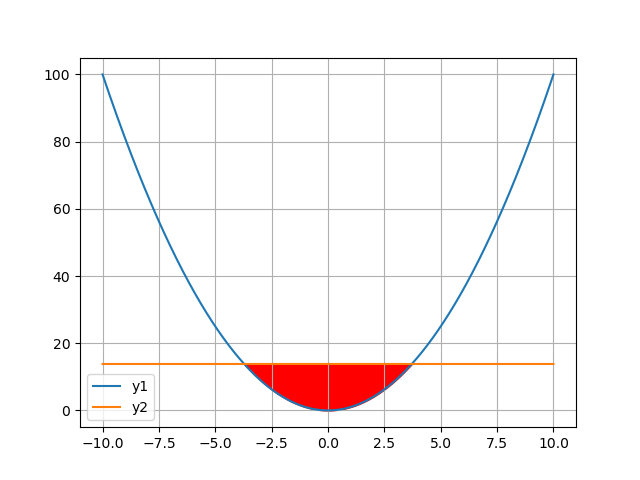
\includegraphics[width=0.6\textwidth]{plot1.png}
    \captionof{figure}{Decision Boundary}
    \begin{flushleft}
        Also, the decision boundary is $R_1 = \{x : -3.72 \leq x \leq 3.72\}$.
    \end{flushleft}
\end{qsolve}
\subsection{b}
Now let $\sigma_{2}^2 = 1$. Once again, find $R_1$ and draw it.
\begin{qsolve}
    \begin{gather*}
        p_X (x|Y=1) \geq p_X(x|Y=2) \\
        \frac{1}{\sqrt{2\pi}} e^{-\frac{1}{2}x^2} \geq \frac{1}{\sqrt{2\pi}} e^{-\frac{1}{2}(x-1)^2} \\
        e^{-\frac{1}{2}x^2} \geq e^{-\frac{1}{2}(x-1)^2} \\
        -\frac{1}{2}x^2 \geq -\frac{1}{2}(x-1)^2 \\
        x^2 \leq (x-1)^2 \\
    \end{gather*}
    \splitqsolve
    To draw the decision boundary, I plot the function $x^2 - (x-1)^2$ via python.
    \begin{lstlisting}[language=Python]
        import numpy as np
        import matplotlib.pyplot as plt
        
        x = np.linspace(-10, 10, 2000)
        y1 = x**2
        y2 = (x-1)**2
        
        plt.plot(x, y1, label='y1')
        plt.plot(x, y2, label='y2')
        plt.fill_between(x, y1, y2, where=y1<y2, color='red')
        plt.grid()
        plt.legend()
        plt.show()        
    \end{lstlisting}
    result : \\ \\
    \centering
    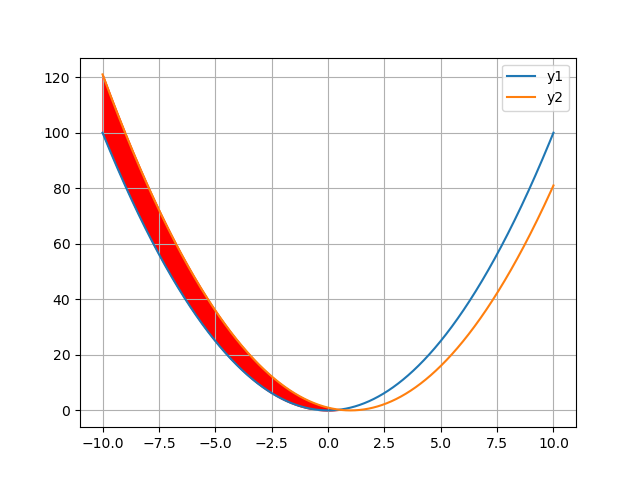
\includegraphics[width=0.6\textwidth]{plot2.png}
    \captionof{figure}{Decision Boundary}
    %start from left
    \begin{flushleft}
        Also, the decision boundary is $R_1 = \{x : x \leq \frac{1}{2}\}$.
    \end{flushleft}
\end{qsolve}

\section{Newton’s Method as Solver For Linear Regression Problem}
In this problem, we will prove that if we use Newton’s method solve the least squares optimization problem, then we only need one iteration to converge to $\theta^{*}$
\subsection{a}
Find the Hessian of the cost function:
\begin{gather*}
    J(\theta) = \frac{1}{2} \sum_{i=1}^{m} (\theta^\top x^{(i)} - y^{(i)})^2
\end{gather*}
\begin{qsolve}
    \begin{gather*}
        J(\theta) = \frac{1}{2} \sum_{i=1}^{m} (\theta^\top x^{(i)} - y^{(i)})^2 \\
        \nabla_\theta J(\theta) = \sum_{i=1}^{m} (\theta^\top x^{(i)} - y^{(i)}) x^{(i)} \\
        \nabla_\theta^2 J(\theta) = \sum_{i=1}^{m} x^{(i)} x^{(i)\top} \\
        \nabla_\theta^2 J(\theta) = X^\top X \\
    \end{gather*}
\end{qsolve}

\subsection{b}
Find the closed form solution for $\Theta^{*}$ which minimizes $J(\theta)$.This is the equivalent to the normal equations for the multivariate case.
\begin{qsolve}
    \begin{gather*}
        \nabla_\theta J(\theta) = 0 \\
        \sum_{i=1}^{m} (\theta^\top x^{(i)} - y^{(i)}) x^{(i)} = 0 \\
        \sum_{i=1}^{m} \theta^\top x^{(i)} x^{(i)} - \sum_{i=1}^{m} y^{(i)} x^{(i)} = 0 \\
        \theta^\top \sum_{i=1}^{m} x^{(i)} x^{(i)} - \sum_{i=1}^{m} y^{(i)} x^{(i)} = 0 \\
        \theta^\top X^\top X - Y^\top X = 0 \\
        \theta^\top X^\top X = Y^\top X \\
        \theta^\top = Y^\top X (X^\top X)^{-1} \\
        \theta = (X^\top X)^{-1} X^\top Y \\
    \end{gather*}
\end{qsolve}

\section{Multivariate Least Squares}
o far in class, we have only considered cases where our target variable $Y$ s a scalar value. Suppose that instead of trying to predict a single output, we have a training set with multiple outputs for each example:
\begin{gather*}
    (\mathbf{x}^{(i)} , \mathbf{y}^{(i)}) , i = 1, . . . , m, \quad \quad \mathbf{x}^{(i)} \in \mathbb{R}^{n}, \mathbf{y}^{(i)} \in \mathbb{R}^{p}
\end{gather*}
Thus for each training example, $\mathbf{y}^{(i)}$ s vector-valued, with p entries. We wish to use a linear model to predict the outputs, as in least squares, by specifying the parameter matrix $\Theta$ in:
\begin{gather*}
    \mathbf{y} = \Theta^\top \mathbf{x}
\end{gather*}
where $\Theta \in \mathbb{R}^{n \times p}$ .
\subsection{a}
The cost function for this case is:
\begin{gather*}
    J(\Theta) = \frac{1}{2} \sum_{i=1}^{m} \sum_{j=1}^{p} (\Theta^\top x^{(i)} - y_j^{(i)})^2
\end{gather*}
write $J(\Theta)$ in matrix-vector notation(i.e. whitout using any without using any summations),
\begin{qsolve}
    \begin{gather*}
        J(\Theta) = \frac{1}{2} \sum_{i=1}^{m} \sum_{j=1}^{p} (\Theta^\top x^{(i)} - y_j^{(i)})^2 \\
        J(\Theta) = \frac{1}{2} \sum_{i=1}^{m} (\Theta^\top x^{(i)} - y^{(i)})^\top (\Theta^\top x^{(i)} - y^{(i)}) \\
        J(\Theta) = \frac{1}{2} \sum_{i=1}^{m} (x^{(i)\top} \Theta - y^{(i)\top}) (x^{(i)} \Theta - y^{(i)}) \\
        J(\Theta) = \frac{1}{2} \sum_{i=1}^{m} (x^{(i)\top} \Theta \Theta^\top x^{(i)} - x^{(i)\top} \Theta y^{(i)} - y^{(i)\top} \Theta^\top x^{(i)} + y^{(i)\top} y^{(i)}) \\
        J(\Theta) = \frac{1}{2} \sum_{i=1}^{m} (x^{(i)\top} \Theta \Theta^\top x^{(i)} - 2 x^{(i)\top} \Theta y^{(i)} + y^{(i)\top} y^{(i)}) \\
        J(\Theta) = \frac{1}{2}  [tr(X \Theta \Theta^\top X^\top) - 2 tr(X \Theta Y^\top) + tr(Y Y^\top)] \\
    \end{gather*}
\end{qsolve}

\subsection{b}
Find the closed form solution for $\Theta^{*}$ which minimizes $J(\theta)$. This is equivalent to the normal equations for the multivariate case.
\begin{qsolve}
    \begin{gather*}
        \nabla_\Theta J(\Theta) = 0 \\
        \nabla_\Theta \frac{1}{2}  [tr(X \Theta \Theta^\top X^\top) - 2 tr(X \Theta Y^\top) + tr(Y Y^\top)] = 0 \\
        \nabla_\Theta \frac{1}{2}  [tr(X \Theta \Theta^\top X^\top)] - \nabla_\Theta \frac{1}{2}  [2 tr(X \Theta Y^\top)] + \nabla_\Theta \frac{1}{2}  [tr(Y Y^\top)] = 0 \\
        \frac{1}{2}  [X^\top X \Theta + X^\top X \Theta] - \frac{1}{2}  [2 X^\top Y] = 0 \\
        X^\top X \Theta = X^\top Y \\
        \Theta = (X^\top X)^{-1} X^\top Y \\
    \end{gather*}
\end{qsolve}

\subsection{c}
Suppose instead of considering the multivariate vectors $y^{(i)}$ all at once, we instead compute each variable($y_{j}^{(i)}$) separately for each $j = 1, 2, \dots, n$. In this case, we have $p$ individual linear models, of the form:
\begin{gather*}
    y_{j}^{(i)} = \theta_{j}^\top x^{(i)} , j = 1, 2, \dots, p
\end{gather*}
(So here, each $\theta_{j} \in \mathbb{R}^{n}$ ). How do the parameters from these $p$ independent least squares problems relate to the parameters $\theta$ from the multivariate least squares problem?
\begin{qsolve}
    \begin{gather*}
        J(\Theta) = \frac{1}{2} \sum_{i=1}^{m} \sum_{j=1}^{p} (\Theta^\top x^{(i)} - y_j^{(i)})^2 \\
        J(\Theta) = \frac{1}{2} \norm{X \Theta - Y}^2 \\
        J(\Theta) = \frac{1}{2} \sum_{i=0}^{p} \norm{X \theta_{i} - Y_{i}}^2 \\
        \argmin_{\Theta} J(\Theta) = \argmin_{\Theta} \frac{1}{2} \sum_{i=0}^{p} \norm{X \theta_{i} - Y_{i}}^2 \\
    \end{gather*}
    we can separate the problem into $p$ independent least squares problems.
    \begin{gather*}
        {\Theta^{*}}^\top = \begin{bmatrix}
            \theta_{1}^{*} \\
            \theta_{2}^{*} \\
            \vdots         \\
            \theta_{p}^{*} \\
        \end{bmatrix}
    \end{gather*}
    where $\theta_{j}^{*}$ is the solution to the $j^{th}$ least squares problem.
\end{qsolve}
\section{Choosing A Proper Mapping}
We have a classification problem where we have a feature vector $\mathbf{x} \in \mathbb{R}^{2}$and two classes (binary classification). Our data is represented as matrices below
\begin{gather*}
    X = \begin{bmatrix}
        4 & 0  \\
        3 & 1  \\
        2 & 0  \\
        3 & -1 \\
        6 & 0  \\
        3 & 3  \\
        0 & 0  \\
        3 & -3 \\
    \end{bmatrix}
    Y = \begin{bmatrix}
        1  \\
        1  \\
        1  \\
        1  \\
        -1 \\
        -1 \\
        -1 \\
        -1 \\
    \end{bmatrix}
\end{gather*}
Find a proper mapping $\phi(\mathbf{x})$ which maps $\mathbf{x}$ to a higher dimensional space such that the data is linearly separable in the introduces space.\\
(Hint: Draw the data points!)
\begin{qsolve}
    I used this python code to find the mapping via drawing the data points:
    \begin{lstlisting}[language=Python]
        import numpy as np
        import matplotlib.pyplot as plt

        X = np.array([
            [4, 0],
            [3, 1],
            [2, 0],
            [3, -1],
            [6, 0],
            [3, 3],
            [0, 0],
            [3, -3],
        ])
        Y = np.array([
            1,
            1,
            1,
            1,
            -1,
            -1,
            -1,
            -1,
        ])

        plt.scatter(X[:, 0], X[:, 1], c=Y)
        plt.show()
    \end{lstlisting}
    result of the code:\\
    \\
    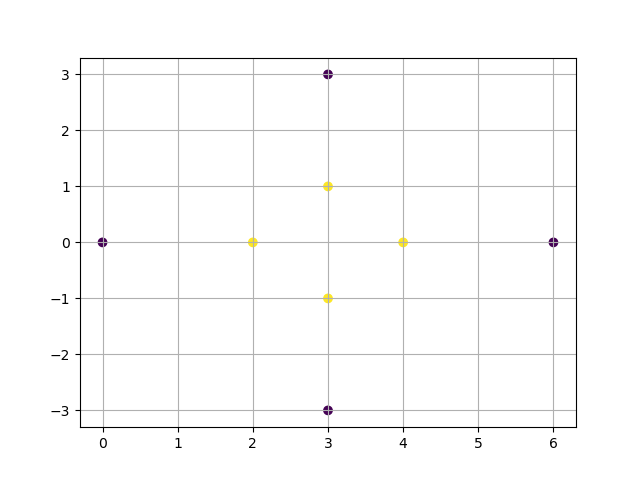
\includegraphics[width=0.5\textwidth]{plot3.png}
    \captionof{figure}{Data points}
    Its obvious that datas which labeled as 1 are on a circle with centre of (3,0) and radius of 3 and datas which labeled as -1 are on a circle with centre of (3,0) and radius of 1.
    So we can map the data to a higher dimensional space with this mapping:
    \begin{gather*}
        \phi(\mathbf{x}) = [x_1,x_2,(x_1-3)^2+{x_2}^2]
    \end{gather*}
\end{qsolve}




















\makeendpage
\end{document}